\section{What limits the advantage in practice}
\label{sec:limits}

The diffusion model's serial advantage is large, but five deployment
factors constrain it in practice.

\paragraph{1. Footprint.}

Both models are MoE with comparable footprints. Neither can share a GPU
with another large model. The asymmetry that matters is against the
quality-similar dense AR-1.5B at 3\,GB: sixteen copies fit in the
space either MoE model occupies.

\paragraph{2. Batching.}

Continuous batching converts arrival concurrency into throughput at
$77\times$ for AR-30B against $\leq 1.7\times$ for DG. We measured
both DG multipliers on engine-bounded stacks, so the true ceiling is
unknown but lies at or above $1.7\times$. Even so, the gap is more
than an order of magnitude; see Appendix~\ref{app:batching}.

\begin{figure}[t]
\centering
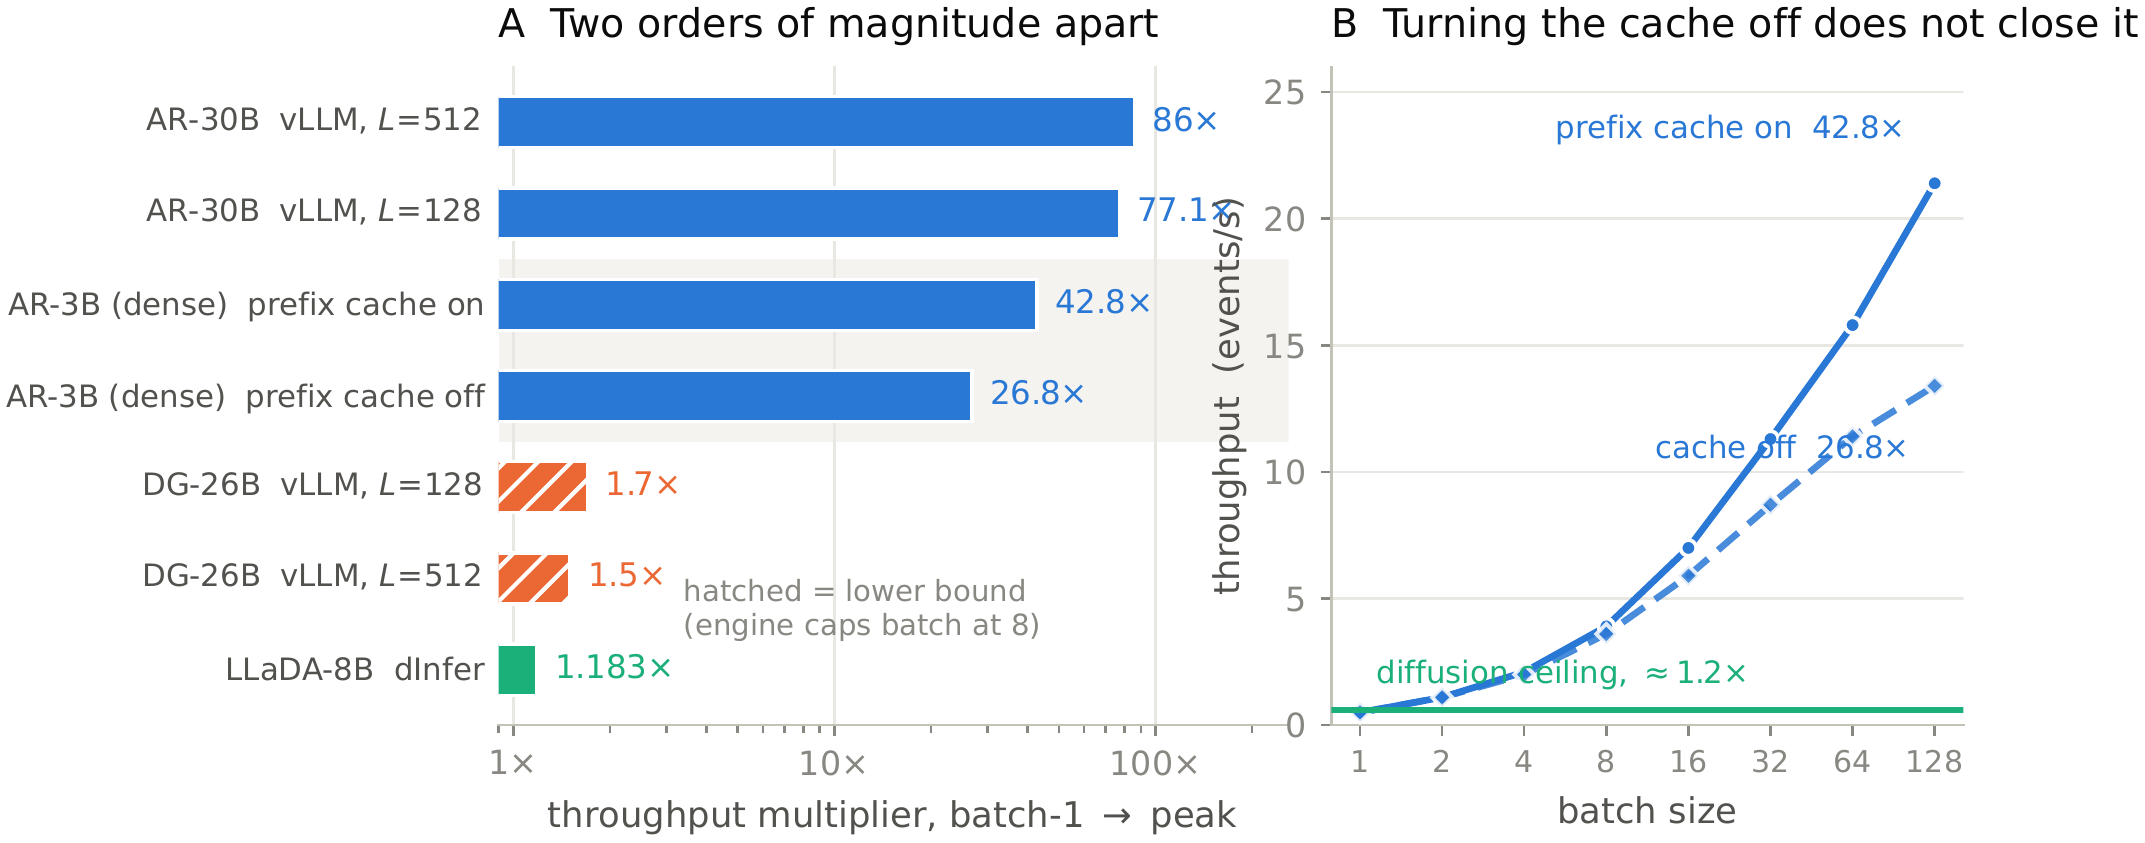
\includegraphics[width=\linewidth]{figures/fig6_batching_hires.png}
\caption{Batch-1 to peak throughput multipliers. AR-30B reaches
$77\times$ via KV-cache reuse; DG caps at $\leq 1.7\times$ because
changing attention masks invalidate KV persistence across denoising
steps. The prefix cache on/off bars are the dense AR-3B, not the
AR-30B MoE (BGL, $n{=}300$).}
\label{fig:batching}
\end{figure}

\paragraph{3. Tail latency.}

The diffusion arm's per-event coefficient of variation is \dgEventCV\%
with a max/median ratio of \dgMaxMed$\times$, against the AR arm's
\arEventCV\% and \arMaxMed$\times$; see Appendix~\ref{app:distributions}.
A $3.21\times$ tail is what breaks a batch-1 SLA --- exactly the
regime where DG's per-event advantage applies.

\paragraph{4. Input length.}

The diffusion prefill slope is \inputSlopeRatio$\times$ steeper than
AR's, because each denoising step re-attends the full prompt. At
longer inputs the base rises and $L^{*}$ moves further upward.

\paragraph{5. Co-residency.}

If batch-1 is imposed by tenant isolation, the relevant alternative is
not the MoE AR-30B but sixteen copies of the quality-similar dense
AR-1.5B. Per-tenant latency is unchanged; throughput is $16\times$;
isolation is preserved.

\paragraph{Cost per event.}

Table~\ref{tab:cost} prices the comparison at a published on-demand
rate. The headline: at full duty, DG processes events at less than a
twentieth of a cent each. The AR-30B costs fifteen times more. For a
B2B log-processing service handling ten thousand events per day, that
is five dollars a day on DG versus seventy-six on AR-30B --- a
\$26{,}000 annual gap on a single GPU.

\begin{table}[h]
\centering
\caption{Cost per event at three duty cycles. GPU: A100 80GB PCIe at
\$4.62/hr (AWS p4de.24xlarge, August 2026).}
\label{tab:cost}
\begin{tabular}{@{}lrrrr@{}}
\toprule
Arm & Weights & Duty & Events/hr & \$/event \\
\midrule
AR-30B MoE (serial) & 60\,GB & 100\% & 610 & \$0.0076 \\
AR-30B MoE           & 60\,GB & 25\%  & 153 & \$0.030 \\
\midrule
AR-1.5B dense (co-resident) & 3.0\,GB & 100\% & 5{,}408 & \$0.0009 \\
AR-1.5B dense                & 3.0\,GB & 25\%  & 1{,}352 & \$0.003 \\
\midrule
DG-26B-A4B (serial)  & 52\,GB & 100\% & 9{,}504 & \$0.0005 \\
DG-26B-A4B            & 52\,GB & 25\%  & 2{,}376 & \$0.002 \\
\bottomrule
\end{tabular}
\end{table}

At full duty on a dedicated GPU, the cost ratio is:
\begin{equation}
R_{\mathrm{cost}} = \frac{\$ / \mathrm{event}_{\mathrm{AR}}}
{\$ / \mathrm{event}_{\mathrm{DG}}}
= \frac{0.0009}{0.0005} = 1.8
\end{equation}
Why does the much slower AR-1.5B nearly match DG on cost? Because at
3\,GB it fits sixteen copies in one GPU, and co-residency is
parallelism by another name. Under co-residency, sixteen AR-1.5B
instances produce $16 \times 5{,}408 = 86{,}528$ events/hr against DG's
9{,}504. The AR co-resident deployment is $9\times$ cheaper per event
while preserving tenant isolation. The honest reading: if you can
batch, AR wins on economics; if you cannot, DG wins on latency.
